\section{%
	\AP\label{sec:dichotomy-colouring}%
	From Separation to Colouring of Automatic Graphs
}

\subsection{Separability is Equivalent to Regular Colourability}

We start by showing that the "separability problem" in terms of arbitrary "recognizable relations" is equivalent, under polynomial time reductions, 
to the "regular colourability problem". To make our statement precise, we need some terminology introduced below. 
\AP
Let $\intro*\kREC$ be the class of languages expressed by unions of products of $k$ regular languages which form a partition, that is (in the binary case), relations of the form $(L_{i_1} \times L_{j_1}) \cup \dotsb \cup (L_{i_\ell} \times L_{j_\ell})$, with $i_1,j_1,\hdots,i_\ell, j_\ell \in \lBrack 1,k \rBrack$, for some regular partition $L_1, \dotsc, L_{k}$ of $\Sigma^*$ and $\ell \in \N$.
\AP
Note that $\REC = \bigcup_k \kREC$.
\AP%
Let us denote by $\intro*\Id$ the identity relation (on any implicit alphabet). Observe that $\Id$ is "automatic" but not "recognizable".

\begin{theorem}
    \AP\label{thm:reg-colourability-equiv-separability}
    There are polynomial-time reductions: 
    \begin{enumerate}
        \item from the "$\REC$-separability problem" to the "regular colourability problem"; 
        \item from the "regular colourability problem" to the "$\REC$-separability problem"; and
        \item from the "$k$-regular colourability problem" to the $\kREC$-"separability problem", for every $k > 0$.
    \end{enumerate}
    Further, the last two reductions are so that the second relation in the instance of the "separability problem" is the identity $\Id$.
\end{theorem}

%The rest of this section is dedicated to proving \Cref{thm:reg-colourability-equiv-separability}.
%\begin{proposition}
   % \AP\label{prop:col-to-sep-reductions}
%    %There are polynomial-time reductions
%    %\begin{enumerate}
%       % \item from the "regular colourability problem" on "automatic graphs" to the $\REC$-"separability problem"; and
%        %\item from the "$k$-regular colourability problem" on "automatic graphs" for every $k \geq 1$ to  the $\kREC$ "separability problem".
%    %\end{enumerate}
%    %Further, the reductions are so that the second relation in the instance of the "separability problem" is the identity $\Id$.
%\end{proposition}

% \change{For the sake of readability, in our proofs, we will assume "wlog" that all "automatic graphs" are defined over $L = \Sigma^*$.}
   
\begin{proof}
   We start with the last two reductions.
    Given an "automatic graph" $\AutGraph{L}{E}$ over an alphabet $\Sigma$, consider the instance $R_1,R_2$ for the $\REC$-"separability problem", where 
    $R_1 = E$ and $R_2 = \Id$. 
    %
    If $\AutGraph{L}{E}$ is "$k$-regular colourable" via the colouring $V_1, \dotsc, V_k$ then the $\kREC$ relation
    $\bigcup_{i \neq j} V_i \times V_j$ separates $R_1$ and $R_2$.
    %
    Conversely, if a $\kREC$ relation $R \subseteq \Sigma^* \times \Sigma^*$ on the partition $V_1 \dcup \dotsb \dcup V_k = \Sigma^*$ separates $R_1$ and $R_2$, then $\bigcup_{i \neq j} V_i \times V_j$ also separates $R_1$ and $R_2$, and this implies that $V_1, \dotsc, V_k$ is a $k$-colouring for $\AutGraph{\Sigma^*}{E}$.
%\end{proof}

\AP For the first reduction, let us introduce some terminology.
Given two relations $R_1,R_2$ over $\Sigma^*$, say that $u \in \Sigma^*$ is ""compatible"" with
$u' \in \Sigma^*$ when for all words $v \in \Sigma^*$:
\begin{center}
    \intro*\compL: $(u,v) \in R_1 \Rightarrow (u',v) \not\in R_2$%
    ,\hphantom{\quad and \quad}
    \intro*\compR: $(v,u) \in R_1 \Rightarrow (v,u') \not\in R_2$,\\
    \intro*\compLpr: $(u',v) \in R_1 \Rightarrow (u,v) \not\in R_2$%
    \hphantom{,}\quad and \quad
    \intro*\compRpr: $(v,u') \in R_1 \Rightarrow (v,u) \not\in R_2$.
\end{center}
\AP
Define the ""incompatibility graph"" $\intro*\incompGraph{R_1}{R_2}$
as the graph whose vertices are all words of $\Sigma^*$,
and with an edge from $u$ to $v$ whenever $u$ is not "compatible" with $v$.
Note that $\incompGraph{R}{\Id}$ is exactly the graph $\AutGraph{\Sigma^*}{R}$.

\begin{example}
	\AP\label{ex:equal_length_plusone}
	Let $\Sigma = \{a,b\}$, $R_1$ be the equal-length relation,
	and
	\[
		R_2 = \{(u, ua) \mid u \in \Sigma^*\} \cup \{(u, ub) \mid u \in \Sigma^*\}.
	\]
	Then, $u$ is "incompatible" with $u'$ if $|u| = |u'|+1$ (this is given by \compL~or \compR),
	or if $|u'| = |u|+1$ (this is given by \compLpr~or \compRpr).
	$R_2$ and the "incompatibility graph" are depicted in \Cref{fig:equal_length_plusone}.
	
	Note that $R_1$ and $R_2$ are separable by the "recognizable" relation
	$S$ consisting of all pairs $(u,v)$ such that $|u|$ and $|v|$ have the same parity.
	Moreover, $\incompGraph{R_1}{R_2}$ is "2-regular colorable", the two colors being
	the words of even and odd length.
 \end{example}
 
\begin{figure}[htb]
	\centering
	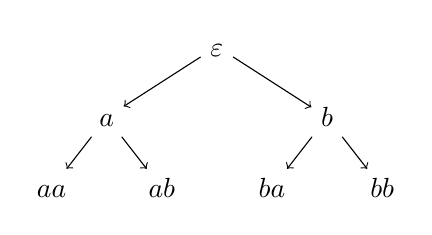
\begin{tikzpicture}
		\tikzset{
	level distance=.9cm,
	level 1/.style={sibling distance=2.8cm},
	level 2/.style={sibling distance=1.4cm},
	level 3/.style={sibling distance=.7cm},
	edge from parent/.style={draw,->}
}

\node (t) {$\varepsilon\vphantom{b}$}
	child {node {$a\vphantom{b}$}
		child {node {$aa\vphantom{b}$}
		}
		child {node {$ab$}
		}
	}
	child {node {$b$}
		child {node {$ba$}
		}
		child {node {$bb$}
		}
	};
	\end{tikzpicture}
	\caption{\AP\label{fig:equal_length_plusone-relation}%
		The relation $R_2$ of \Cref{ex:equal_length_plusone},
		restricted to words of length at most 2.
	}
\end{figure}

\begin{figure}[htb]
	\centering
	\begin{tikzpicture}
		\tikzset{
	level distance=.9cm,
	level 1/.style={sibling distance=2.8cm},
	level 2/.style={sibling distance=1.4cm},
	level 3/.style={sibling distance=.7cm},
	edge from parent/.style={}
}

% Coloring
\fill[rounded corners, fill=cBlue, opacity=.5]
	(-2.5,-2.05) rectangle (2.5,-1.57)
	(-.3,-0.25) rectangle (.3,0.23);
\fill[rounded corners, fill=cYellow, opacity=.5]
	(-1.65,-1.15) rectangle (1.65,-0.67);
% Tree
\node (eps) {$\varepsilon\vphantom{b}$}
	child {node (a) {$a\vphantom{b}$}
		child {node (aa) {$aa\vphantom{b}$}
		}
		child {node (ab) {$ab$}
		}
	}
	child {node (b) {$b$}
		child {node (ba) {$ba$}
		}
		child {node (bb) {$bb$}
		}
	};
\draw[<->] (eps) edge (a)
	(eps) edge (b)
	(a) edge (aa)
	(a) edge (ab)
	(a) edge (ba)
	(a) edge (bb)
	(b) edge (aa)
	(b) edge (ab)
	(b) edge (ba)
	(b) edge (bb);
	\end{tikzpicture}
	\caption{\AP\label{fig:equal_length_plusone-incompatibility}%
		Incompatibility graph $\incompGraph{R_1}{R_2}$ and its "2-regular coloring".
	}
 \end{figure}

\begin{lemma}
    \AP\label{lem:incomp-is-automatic}
    If $R_1$ and $R_2$ are "automatic", then so is $\incompGraph{R_1}{R_2}$.
    Moreover, we can build an automaton for $\incompGraph{R_1}{R_2}$ in polynomial time in the size of the automata for $R_1$ and $R_2$.
\end{lemma}
\begin{proof}
    By definition, the "incompatibility relation" $\incompGraph{R_1}{R_2}$ can be written as
	$R_{\neg\compL} \cup R_{\neg\compLpr} \cup R_{\neg\compR} \cup R_{\neg\compRpr}$, where:
	\begin{align*}
        R_{\neg\compL} &\defeq \big\{ (u,u') \in \Sigma^* \times \Sigma^* \;\big\vert\; \exists v \in \Sigma^*,\; (u,v) \in R_1 \land (u',v) \in R_2 \big\} \text{,}\\
        R_{\neg\compLpr} &\defeq \big\{ (u,u') \in \Sigma^* \times \Sigma^* \;\big\vert\; \exists v \in \Sigma^*,\; (u',v) \in R_1 \land (u,v) \in R_2 \big\} \text{,}\\
        R_{\neg\compR} &\defeq \big\{ (u,u') \in \Sigma^* \times \Sigma^* \;\big\vert\; \exists v \in \Sigma^*,\; (v,u) \in R_1 \land (v,u') \in R_2 \big\} \text{, and}\\
        R_{\neg\compRpr} &\defeq \big\{ (u,u') \in \Sigma^* \times \Sigma^* \;\big\vert\; \exists v \in \Sigma^*,\; (v,u') \in R_1 \land (v,u) \in R_2 \big\}
    \end{align*}
    % % \end{itemize}
    % \begin{itemize}
    %     \item $\neg$\compL:  $(u,v) \in R_1$ and $(u',v) \in R_2$, or
    %     \item $\neg$\compLpr: $(u',v) \in R_1$ and $(u,v) \in R_2$, or
    %     \item $\neg$\compR: $(v,u) \in R_1$ and $(v,u') \in R_2$, or
    %     \item $\neg$\compRpr: $(v,u') \in R_1$ and $(v,u) \in R_2$.
    % \end{itemize} 
    Observe that starting from automata for $R_1$ and $R_2$, then for each
	of the relation $R_{\neg\compL}$, $R_{\neg\compLpr}$, $R_{\neg\compR}$ or $R_{\neg\compRpr}$, we can build an automaton recognizing them
	using a product construction, which can be implemented in polynomial time.
    % as follows:
    % \begin{itemize}
    %     \item its states are $Q_1 \times Q_2$;
    %     \item for each transition $q_1 \xrightarrow{(a,b)} q'_1$ in $\+A_1$
    %         and each transition $q_2 \xrightarrow{(c,b)} q'_2$ in $\+A_2$,
    %         put a transition $(q_1,q_2) \xrightarrow{(a,c)} (q'_1,q'_2)$,
    %         with $a,b,c \in \A\cup\{\bot\}$;\footnote{Potentially, this
    %         could produced transition labelled by $(\bot,\bot)$: we can get rid of those
    %         using the standard elimination of $\varepsilon$-transitions.}
    %     \item a state $(q_1,q_2)$ is accepting if $q_1$ and $q_2$ are accepting
    %         in $\+A_1$ and $\+A_2$, respectively.
    % \end{itemize}
    It then follows that we can build a polynomial automaton recognizing
    $\incompGraph{R_1}{R_2}$.
\end{proof}

%\begin{proposition}
%    \AP\label{prop:sep-to-col-reduction}
%    There is a polynomial-time reduction
%    from the $\REC$-"separability problem" to the 
%    "regular colourability problem" on "automatic graphs".
%\end{proposition}

%\begin{proof}
    \AP Given an instance $(R_1,R_2)$ of the "separability problem", we
    reduce it to the "regular colourability problem" on its "incompatibility graph" $\incompGraph{R_1}{R_2}$.

    \proofcase{Left-to-right implication:} 
   Assume that there exists $S$ in $\kREC$ that "separates" $R_1$ from $R_2$.
   %, where each $A_i$ and $B_i$ is regular.
    Then $S$ can be written as $(A_{i_1}\times A_{j_1}) \cup \cdots \cup (A_{i_\ell}\times A_{j_\ell})$, 
    where $(A_1,\hdots,A_k)$ is a partition of $\Sigma^*$ in $k$ regular languages.
   We define the colour of a word $u \in \Sigma^*$ as the unique $i \in \lBrack 1,k \rBrack$
    "st" $u \in A_i$. In other words, the colouring is simply $(A_1,\hdots,A_k)$. 

    This is indeed a proper colouring: if $u$ and $u'$ have the same colour,
    we claim that $u$ is "compatible" with $u'$. Indeed, take any $v \in \Sigma^*$: if $(u,v) \in R_1$,
    then $(u,v) \in S$, so $(u,v) \in A_{i_m}\times A_{j_m}$ for some $m$. But since $u$ has the same colour 
    as $u'$, the fact that $u \in A_{i_m}$ implies $u' \in A_{i_m}$, and hence 
    $(u',v) \in A_{i_m}\times A_{j_m}\subseteq S$.
    But $S$ separates $R_1$ from $R_2$, and therefore $(u',v) \not\in R_2$. This tells us that \compL\ holds. 
    The other conditions hold by symmetry.
    We conclude that $(A_1,\hdots,A_k)$ defines
    a proper colouring of $\incompGraph{R_1}{R_2}$, and this colouring, with $k$ colours, is 
    "regular@regular colouring" since the $A_i$'s are regular languages by definition.

    \proofcase{Right-to-left implication:} Assume that $\incompGraph{R_1}{R_2}$ is finitely colourable, say by
    $(A_1,\hdots,A_k)$. Then let $S$ be the union of all $S_i$'s where
    \begin{align*}
        S_{i} & \defeq \{(u,v) \mid u \in A_i \text{ and } (u',v) \in R_1 \text{ for some } u' \in A_i \}\\
&         \hphantom{\defeq~}\cup \{(u,v) \mid v \in A_i \text{ and } (u,v') \in R_1 \text{ for some } v' \in A_i \}.  
    \end{align*}
    Since $(A_1,\hdots,A_k)$ covers every node of $\incompGraph{R_1}{R_2}$, we get $R_1 \subseteq S$.
    Moreover, we claim that $R_2 \cap S = \emptyset$. Indeed, if $(u,v) \in S$,
    then $(u,v) \in S_{i}$ for some $i,j$. It either means that \proofcase{1}
    $(u',v) \in R_1$ for some $u' \in A_i$, or \proofcase{2} $(u,v') \in R_2$
    for some $v' \in A_i$. In case \proofcase{1}, the fact that $u \in A_i$ implies that $u$ and $u'$
    have the same colour. Thus, $u$ must be "compatible" with $u'$ and hence
    $(u,v) \not\in R_2$ using \compLpr. The other case is symmetric.
    Therefore, $(u,v) \not\in R_2$, and thus $S$ separates $R_1$ from $R_2$.

    Finally,  $S$ is "recognizable"; in fact, 
    $S = \bigcup_{i=1}^k \bigl( A_i \times R_1[A_i] \bigr) \cup \bigl( R_1^{-1}[A_i] \times A_i \bigr)$, 
    where for any set $X \subseteq \Sigma^*$ we define $R_1[X]$ (resp. $R_1^{-1}[X]$) as the set
    of $v\in \Sigma^*$ (resp. $u \in \Sigma^*$) such that $(u,v) \in R_1$ for some $u \in X$
    (resp. $v\in X$).
    Hence, $R_1$ and $R_2$ are $\REC$-"separable". 
\end{proof}

% \begin{theorem} 
% The following statements hold: 
% \begin{enumerate} 
% \item There is an algorithm that takes as input an automatic relation $L$, and computes two "automatic relations" $L_1$ and $L_2$
% such that 
% $L_1$ is separable from $L_2$ by some recognizable relation $R$ iff ${\cal G}_L$ is finitely colourable with regular colours.
% \item There is an algorithm that takes as input two "automatic relations" $L_1$ and $L_2$, and computes an automatic relation $L$ such that 
% $L_1$ is separable from $L_2$ by some recognizable relation $R$ iff ${\cal G}_L$ is finitely colourable with regular colours. 
% \end{enumerate} 
% \end{theorem}

% \begin{proof} 
% For (1), .

% \medskip 

% For (2), let us assume that $L_1$ and $L_2$ are over alphabet $\Sigma$. We 
% call two words $w,w' \in \Sigma^*$ {\em compatible under $(L_1,L_2)$}, if the following statements hold 
% for every $u \in \Sigma^*$:  
% \begin{itemize} 
% \item 
% If $(w,u) \in L_1$ then $(w',u) \not\in L_2$. 
% \item 
% If $(w',u) \in L_1$ then $(w,u) \not\in L_2$. 
% \item 
% If $(u,w) \in L_1$ then $(u,w') \not\in L_2$. 
% \item 
% If $(u,w') \in L_1$ then $(u,w) \not\in L_2$. 
% \end{itemize} 
% Notice that the compatibility relation under $(L_1,L_2)$ over $\Sigma^*$, denoted $\sim$, 
% is reflexive and symmetric but not necessarily transitive.  
% %Moreover, it is a binary regular relation
% We write ${\cal G}^{\not\sim}_{(L_1,L_2)}$ for the undirected graph defined {\em by the complement} of the compatibility relation under $(L_1,L_2)$ over $\Sigma^*$.  
% It is easy to see that ${\cal G}^{\not\sim}_{(L_1,L_2)}$ is an automatic graph. 

% We claim that the following are equivalent: 
% \begin{itemize} 
% \item 
% $L_1$ is separable from $L_2$ by some recognizable relation $R$. 
% \item ${\cal G}^{\not\sim}_{(L_1,L_2)}$ is finitely colourable with regular colours. 
% \end{itemize} 
% Assume, on the first hand, that $G^{\not\sim}_{(L_1,L_2)}$ can be coloured with finitely many colours $\{0,\dots,k\}$ and that 
% the set $S_i$ of words coloured $i$ is in regular, for each $i \in [0,k]$. 
% Then $S_i$ defines an independent set of the graph, i.e., all words in $S_i$ 
% are mutually compatible under $(L_1,L_2)$.
% We write ${\sf Adj}(S_i)$ for the set of indexes $j \leq k$ such that for some word $u \in S_i$ there is a word $w \in S_j$ with $(u,w) \in L_1$. 
% Let us define $$R \ = \ \bigcup_{i}^k \bigcup_{j \in {\sf Adj}(S_i)} S_i \times S_j.$$  
% Clearly, $R$ is a recognizable relation as each $S_i$ is a regular language. 
% We prove next that $R$ separates $L_1$ from $L_2$.  
% %Let us define a binary relation 
% %%\begin{multline*} 
% %$$E_i \, := \, \{ (\bar w,\bar u) \, \mid \, \bar w \in S_i \text{ and } (\bar w',\bar u) \in L \text{ for some $\bar w' \in S_i$}\}.$$ 
% %%\, \cup \\ 
% %%\{ (\bar u,\bar w) \, \mid \, \bar w \in S_i \text{ and } (\bar u,\bar w') \in L \text{ for some $\bar w' \in S_i$}\}. 
% %%\end{multline*} 
% %Let us also define $R := E_1 \cup \dots \cup E_k$. 
% %Notice that each $E_i$ is regular relation, and hence $R$ is a regular relation. 
% In fact, $L_1 \subseteq R$ as for each word $w$ that appears in $G^{\not\sim}_{(L_1,L_2)}$ we have that, if $w \in S_i$ for $i \leq k$, then 
% $\{(w,u) \mid (w,u) \in L_1\} \subseteq \bigcup_{j \in {\sf Adj}(S_i)} S_i \times S_j$. 
% Moreover, $R \cap L_2 = \emptyset$. This follows directly from the definition of compatibility. In fact, if 
% $(w,u) \in R$ then $(w,u) \in S_i \times S_j$, for some $i,j \leq k$ with $j \in {\sf Adj}(S_i)$, and hence 
% by definition we have that $w \in S_i$ and $(w',u) \in L_1$, for some $w' \in S_i$ and $u \in S_j$.
% \remi{I think it's false: it means $(w',u') \in L_1$, for some $w' \in S_i$ and $u' \in S_j$.} 
% As mentioned above, $w$ and $w'$ are compatible under $(L_1,L_2)$. Hence, $(w,u) \not\in L_2$ by definition.  
 
% %It remains to show that $R$ 
% %is a recognizable relation. In order to prove this it suffices to show that 
% %each $E_i$ is a finite union of products of regular languages. This follows directly from the self-evident claim that 
% %$E_i = \bigcup_{j = 1}^k S_i \times S_j^{\overrightarrow{S_i,L}}$, for each $i \leq k$, 
% %and the fact that $S_i,S_j \in \cal C$ by assumption, and hence $S_j^{\overrightarrow{S_i,L}} \in \C$ since $\C$ is closed under synchronized projections.   

% Assume, in turn, that $L_1$ and $L_2$ are separable by the recognizable relation $R = \bigcup_{i = 1}^k A_i \times B_i$.
% %, where 
% %each $R_i$ is a finite conjunction of expressions of the form $A \times B$ or $\neg (A \times B)$, with $A,B \in \cal C$. 
% %We assume without loss of generality that the $R_i$'s are nonempty.  
% %Notice that, since $\C$ is closed under Boolean combinations, we can assume that each $R_i$ is of the form $A_i \times B_i$, for $A_i,B_i \in \C$. 
% %We can safely assume that the products $A_i \times B_i$ define a partition of $R$, i.e., no pair $(u,v) \in R$ satisfies that 
% %$(u,v) \in A_i \times B_i$ and $(u,v) \in A_j \times B_j$ for $1 \leq i < j \leq k$. 
% For each $X \subseteq [1,k]$ we define a colour $c_X$, and colour with it all words $u \in G^{\not\sim}_{(L_1,L_2)}$ such that $X$ is  
% the set of indices $i \leq k$ for which there is a $w \in \Sigma^*$ with $(u,w) \in A_i \times B_i$. 
% Clearly, the set of words coloured $c_X$ is regular. 
% We claim that it is also a proper colouring of the graph. For that, we prove that if words $u,v$ both receive colour $c_X$ then they must 
% be compatible under $(L_1,L_2)$. Consider an arbitrary word $w$ such that $(u,w) \in L_1$. Then $(u,w) \in R$ as $L_1 \subseteq R$ by assumption, 
% and hence $(u,w) \in A_i \times B_i$ for some $i \in X$. 
% By definition, there is also a word $w'$ such that $(v,w') \in A_i \times B_i$. Hence $(v,w) \in A_i \times B_i \subseteq R$,
% from which we conclude that $(v,w) \not\in L_2$ since $L_2 \cap R = \emptyset$ by assumption. 
% All other cases are symmetric. 
% %To finalize, we need to show 
% %that the set of words coloured with $c_X$, for each $X \subseteq [1,k]$, is regular. 
% %Since $\C$ is closed under Boolean combinations, 
% %it suffices to show that for each $i \leq k$ 
% %the set of words $\bar u \in \Sigma^*$ for which $(\bar u,\bar w) \in R_i = A_i \times B_i$, for some $\bar w \in \Sigma^*$, is in $\C$. 
% %But this set is precisely $A_i$, which is in $\C$ by assumption.  
% \end{proof} 

It is not known to date whether the "regular colourability problem" is decidable, and hence 
the same holds for the $\REC$-"separability problem"
in light of the previous theorem. This is due to the fact that there are no known characterizations of when an "automatic graph" is finitely colourable. 
In spite of this, we believe that the connection between separability and finite colourability is of interest, as it provides us with a way to define and study meaningful 
restrictions of our problems. The first such restriction corresponds to the "$k$-regular colourability problem" for "automatic graphs", which we study in the next section. 

\subsection{$k$-Regular Colourability Problem}

While we do not know how to approach the "regular colourability problem", we show that as soon as we add the restriction that the number of colours is bounded, the problem becomes undecidable; i.e., the "$k$-regular colourability problem" is undecidable for $k\geq 2$. Using this, we obtain in the next section 
the undecidability for the "separability problem" on two natural classes of 
"recognizable relations". This is proven by a reduction from a suitable problem on reversible 
Turing Machines with certain restrictions, which we call ``well-founded''.

\subsection{Regularity of Reachability for Turing Machines}
We use the standard notation $u[i..j]$ to denote the factor of a word $u$ between (and including) positions $i$ and $j$, and $u[i]$ to denote $u[i..i]$.
%\sidediego{Should this go the preliminaries?}
Consider any deterministic Turing Machine (TM) $T = \tup{Q,\Gamma,\bot,\delta,q_0,F}$, where $Q$ is the set of states, $\Gamma$ is tape alphabet, $\bot$ is the blank symbol, $\delta: (Q \setminus F) \times \Gamma_\bot \to Q \times \Gamma \times \set{L,R}$ is the transition (partial) function, where $\Gamma_\bot = \Gamma \cup \set\bot$, and $q_0$ and $F$ is the initial and set of final states, respectively.
%
We represent a configuration with tape content $w \cdot \bot^\omega$ (where $w \in \Gamma^* \cdot \set{\bot}$), in state $q$ and with the head pointing to the cell number $1 \leq i \leq |w|$, as the string
\[
   w[1..i-1] \cdot (w[i],q) \cdot w[i+1..|w|] 
\]
over the alphabet $\Sigma_T = \Gamma \cup (\Gamma_\bot \times Q)$.
\AP In light of this representation, we will henceforth denote by ``configuration'' any string from the set  $\intro*\configs \defeq (\Gamma^* \cdot (\Gamma_\bot \times Q)) \cup  (\Gamma^* \cdot (\Gamma \times Q) \cdot \Gamma^*)$. The ""initial configuration"" is $(\bot,q_0)$.
\AP The ""configuration graph"" of $T$ is the infinite graph $\intro*\confGraph$ having $\configs$ as set of vertices and an edge from $c$ to $c'$, denoted $c \rightarrow c'$, if $c'$ is the configuration of the next step of $T$ starting from $c$. Observe that the "configuration graph" $\confGraph$ of any TM $T$ is an effective "automatic graph" (see, e.g., \cite{KL10}).

\AP We say that a deterministic TM $T$ is ""reversible"" if every node of $\confGraph$ has in-degree at most 1, in other words if the machine is co-deterministic\footnote{Note
that a modern proof of undecidability of the isomorphism problem for automatic structures by
Blumensath \cite[\S VIII. Theorem 4.3, p. 396 \& second claim, p. 398]{blumensath2023MSO} also relies on the use of "reversible" Turing machines.}.
We say that a TM $T$ is a ""well-founded Reversible Turing Machine"" (\reintro{wf-RTM}) if its "configuration graph" is such that (1) the "initial configuration" has in-degree 0 (2) every node has in-degree and out-degree at most one (3) there are no infinite backward paths $c_1 \leftarrow c_2 \leftarrow \dotsb$ in $\confGraph$. 

\AP Note that every "well-founded Reversible Turing Machine" is deterministic and "reversible" and, moreover,
its "configuration graph" is a (possibly infinite) disjoint union of
directed paths, which are all finite, or isomorphic to $(\mathbb{N}, +1)$.
The set of ""reachable configurations"", denoted by $\intro*\Reach$, is 
the set of all configurations that admit a path from the "initial configuration"
% the set of all "configurations" in the connected component of the "initial configuration" 
in $\confGraph$, for a given TM $T$.
Such a configuration graph is depicted on \Cref{subfig:config-graph-wf-RTM}.

\AP The ""reachable regularity problem"" is the problem of, given a "wf-RTM" $T$, whether its set of "reachable configurations" is a regular language. To show that is it undecidable, we exhibit a reduction from the halting problem on deterministic "reversible" Turing machines.

\begin{proposition}[{\cite[Theorem 1]{lecerf1963machines}}]
    \AP\label{prop:halting-problem-detrevTM}
    The halting problem on deterministic "reversible" Turing machines is undecidable.
\end{proposition}

For more details and pointers on "reversible" Turing machines, see \cite[Chapter 5]{Morita2017}.

\begin{lemma}
    \AP\label{lem:reachable-regularity}
    The "reachable regularity problem" is undecidable.
\end{lemma}

\begin{proof}[Proof sketch]
    By reducing the halting problem on deterministic "reversible" Turing machines,
    in such a way that the "reachable configurations" whose
    state $q$ coincide with the state of the original machine are
    of the form $(u q v a^n b^n)$ where $(u q v)$ is a configuration of the original machine,
    $a$ and $b$ are new symbols,
    and $n\in\N$. Transitions are defined in such a way that the new machine is a
    "wf-RTM": this is implemented by having, for every transition $uqv \to u'q'v'$ of the original machine and every $n\in \N$, a (multi-step) transition $(u q v a^n b^n) \to^* (u' q' v' a^{n+1} b^{n+1})$---and is illustrated in \Cref{fig:reachable-regularity}.
	\begin{figure}[htb]
		\centering
		\begin{tikzpicture}
			% ---
% First tape
% ---
\node (0) at (0,0) {0};
\node[right = 0cm of 0] (1) {0};
\node[right = 0cm of 1] (2) {1};
\node[right = 0cm of 2] (3) {0};
\node[right = 0cm of 3] (4) {1};
\node[right = 0cm of 4] (5) {$a\vphantom{b}$};
\node[right = 0cm of 5] (6) {$a\vphantom{b}$};
\node[right = 0cm of 6] (7) {$a\vphantom{b}$};
\node[right = 0cm of 7] (8) {$b$};
\node[right = 0cm of 8] (9) {$b$};
\node[right = 0cm of 9] (10) {$b$};

\draw[rounded corners=4pt] (0.south west) rectangle (10.north east);
\draw[->, thick] ($(5.north)+(0,.4)$) -- ($(5.north)+(0,.1)$);
\node[above=.05cm, circle, draw=cBlue, fill=cBlue, opacity=.5, text opacity=1, inner sep=1.5pt] at ($(5.north)+(0,.4)$) {$p$};

% ---
% Second tape
% ---
\node[below = 1.2cm of 0] (0') {0};
\node[right = 0cm of 0'] (1') {0};
\node[right = 0cm of 1'] (2') {1};
\node[right = 0cm of 2'] (3') {0};
\node[right = 0cm of 3'] (4') {1};
\node[right = 0cm of 4'] (5') {1};
\node[right = 0cm of 5'] (6') {$a\vphantom{b}$};
\node[right = 0cm of 6'] (7') {$a\vphantom{b}$};
\node[right = 0cm of 7'] (8') {$b$};
\node[right = 0cm of 8'] (9') {$b$};
\node[right = 0cm of 9'] (10') {$b$};

\draw[rounded corners=4pt] (0'.south west) rectangle (10'.north east);
\draw[->, thick] ($(6'.north)+(0,.4)$) -- ($(6'.north)+(0,.1)$);
\node[above=.05cm, circle, draw=cRed, fill=cRed, opacity=.5, text opacity=1, inner sep=1.5pt] at ($(6'.north)+(0,.4)$) {$\phantom{q}$};

% ---
% Third tape
% ---
\node[below = 1.2cm of 0'] (0'') {0};
\node[right = 0cm of 0''] (1'') {0};
\node[right = 0cm of 1''] (2'') {1};
\node[right = 0cm of 2''] (3'') {0};
\node[right = 0cm of 3''] (4'') {1};
\node[right = 0cm of 4''] (5'') {1};
\node[right = 0cm of 5''] (6'') {$a\vphantom{b}$};
\node[right = 0cm of 6''] (7'') {$a\vphantom{b}$};
\node[right = 0cm of 7''] (8'') {$a\vphantom{b}$};
\node[right = 0cm of 8''] (9'') {$a\vphantom{b}$};
\node[right = 0cm of 9''] (10'') {$b$};

\draw[rounded corners=4pt] (0''.south west) rectangle (10''.north east);
\draw[->, thick] ($(10''.north)+(0,.4)$) -- ($(10''.north)+(0,.1)$);
\node[above=.05cm, circle, draw=cRed, fill=cRed, opacity=.5, text opacity=1, inner sep=1.5pt] at ($(10''.north)+(0,.4)$) {$\phantom{q}$};

% ---
% Fourth tape
% ---
\node[below = 1.2cm of 0''] (0''') {0};
\node[right = 0cm of 0'''] (1''') {0};
\node[right = 0cm of 1'''] (2''') {1};
\node[right = 0cm of 2'''] (3''') {0};
\node[right = 0cm of 3'''] (4''') {1};
\node[right = 0cm of 4'''] (5''') {1};
\node[right = 0cm of 5'''] (6''') {$a\vphantom{b}$};
\node[right = 0cm of 6'''] (7''') {$a\vphantom{b}$};
\node[right = 0cm of 7'''] (8''') {$a\vphantom{b}$};
\node[right = 0cm of 8'''] (9''') {$a\vphantom{b}$};
\node[right = 0cm of 9'''] (10''') {$b$};
\node[right = 0cm of 10'''] (11''') {$b$};
\node[right = 0cm of 11'''] (12''') {$b$};
\node[right = 0cm of 12'''] (13''') {$b$};

\draw[rounded corners=4pt] (0'''.south west) rectangle (13'''.north east);
\draw[->, thick] ($(13'''.north)+(0,.4)$) -- ($(13'''.north)+(0,.1)$);
\node[above=.05cm, circle, draw=cRed, fill=cRed, opacity=.5, text opacity=1, inner sep=1.5pt] at ($(13'''.north)+(0,.4)$) {$\phantom{q}$};

% ---
% Fifth tape
% ---
\node[below = 1.2cm of 0'''] (0'''') {0};
\node[right = 0cm of 0''''] (1'''') {0};
\node[right = 0cm of 1''''] (2'''') {1};
\node[right = 0cm of 2''''] (3'''') {0};
\node[right = 0cm of 3''''] (4'''') {1};
\node[right = 0cm of 4''''] (5'''') {1};
\node[right = 0cm of 5''''] (6'''') {$a\vphantom{b}$};
\node[right = 0cm of 6''''] (7'''') {$a\vphantom{b}$};
\node[right = 0cm of 7''''] (8'''') {$a\vphantom{b}$};
\node[right = 0cm of 8''''] (9'''') {$a\vphantom{b}$};
\node[right = 0cm of 9''''] (10'''') {$b$};
\node[right = 0cm of 10''''] (11'''') {$b$};
\node[right = 0cm of 11''''] (12'''') {$b$};
\node[right = 0cm of 12''''] (13'''') {$b$};

\draw[rounded corners=4pt] (0''''.south west) rectangle (13''''.north east);
\draw[->, thick] ($(6''''.north)+(0,.4)$) -- ($(6''''.north)+(0,.1)$);
\node[above=.05cm, circle, draw=cBlue, fill=cBlue, opacity=.5, text opacity=1, inner sep=1.5pt] at ($(6''''.north)+(0,.4)$) {$q$};

% ---
% Transitions
% ---
\draw[->, dashed] ($(10.east)+(.3,-.2)$) to[bend left=50]
	node[midway, right=.15cm, align=left, text width=3.5cm, font=\footnotesize] {simulate $T$}
	($(10'.east)+(.3,.2)$);

\draw[->, dashed] ($(10'.east)+(.3,-.2)$) to[bend left=50]
	node[midway, right=.15cm, align=left, text width=3.5cm, font=\footnotesize]
		{overwrite the first two $b$'s with $a$'s}
	($(10''.east)+(.3,.2)$);

% \draw[-, dashed] ($(10''.east)+(.3,-.1)$) to ($(10''.east)+(1.5,-.1)$);
\draw[->, dashed] ($(10''.east)+(1.5,-.2)$) to[bend left=50]
	node[midway, right=.15cm, align=left, text width=3.5cm, font=\footnotesize]
		{append three $b$'s}
	($(13'''.east)+(.3,.2)$);


\draw[->, dashed] ($(13'''.east)+(.3,-.2)$) to[bend left=50]
	node[midway, right=.15cm, align=left, text width=3.5cm, font=\footnotesize]
		{go back to the new position, in the new state}
	($(13''''.east)+(.3,.2)$);
		\end{tikzpicture}
		\caption{
			\AP\label{fig:reachable-regularity}
			Encoding of a single transition of the form
			``when reading a blank in state $\color{cBlue} p$, write a
			$1$, go in state $\color{cBlue} q$ and move right''
			of the machine $T$ in the machine $T'$
			in the proof of \Cref{lem:reachable-regularity}.
			Red unlabelled states represent states of $T'$
			that are not originally present in $T$.
		}
	\end{figure}
	Moreover:
    \begin{itemize}
        \item if the original machine was halting, then the "reachable configurations"
            of the new one are finite and hence regular;
        \item otherwise, the set of "reachable configurations" is not regular,
            which follows from the non-regularity of any infinite subset of $\{a^n b^n \mid n \in \N\}$.
    \end{itemize}
\end{proof}

\begin{proof}
    By reduction from the halting problem for deterministic and "reversible" TMs, which is undecidable by \Cref{prop:halting-problem-detrevTM}. Given a deterministic and "reversible" TM $T$ (running on the empty input), consider the TM $T'$ where every time there is a transition $(u, p, v) \to (u', q, v')$ from configuration $c$ to configuration $c'$ in $T$,
	simulate this transition in $T'$---$a$'s should be treated as blank symbols---,
	and then rewrite $a^n b^n$ into $a^{n+1}b^{n+1}$.
	When $T$ writes on a blank symbol that was actually a $a$ in $T'$,
	we must also add an extra $a$ (to account for the one that was overwritten):
	this case is depicted \Cref{fig:reachable-regularity}.
	Moreover, when $T$ deletes a symbol at the end of the tape,
	we must shift the $a^n b^n$ prefix. This can be done by replacing the blank
	with an $a$, the last $a$ with a $b$, and deleting the last $b$.
	
	% in \Cref{fig:reachable-regularity}, by a series of steps that ``make some room'' between $c$ and $c'$ if needed (for example because the head was at the last position of $c$ and moves to the right), and make some room between the $a$'s and the $b$'s to accomodate for the extra $a$, and writes an extra $b$ at the end. This can be done with the invariant that at all times there are roughly as many $a$'s as $b$'s ($\pm 1$) in the working tape.
    Observe that $T'$ is a "wf-RTM":
    \begin{enumerate}
        \item the "initial configuration" $(\bot,q_0,\bot)$ has no predecessor;
        \item it is deterministic and co-deterministic:
        \begin{itemize}
            \item every configuration inside a path $(u, q, v a^n b^n) \xrightarrow{*} (u, q, v a^{n+1} b^{n+1})$ 
            has, by definition, exactly in- and out-degree one;
            \item every configuration of the form $(u, p, v a^n b^n)$ has as many predecessors [resp.  
                successors] in $T'$ as $(u,q,v)$ in $T$, namely one since $T$ was assumed to be
                deterministic and "reversible";
        \end{itemize}
        \item it has no infinite descending chain since $\N$ is well-founded.
    \end{enumerate}
    Moreover $T'$ has no cycle,
    so if $T$ is halting (on an empty input) then the set of "reachable configurations" of $T'$ is finite (since it is a "wf-RTM") and thus regular. If $T$ is not halting, the set of "reachable configurations" of $T'$ is infinite and its projection onto $\set{a,b}$ is an infinite set of words of the form $a^{n} b^{n'}$ where $n-2 \leq n' \leq n+2$. Hence, since regular languages are closed under homomorphic images, the "reachable configurations" of $T'$ cannot be regular.
\end{proof}



\subsection[Undecidability of the $k$-Regular colourability Problem]{Undecidability of the $\boldsymbol{k}$-Regular colourability Problem}
We can now show undecidability for the "$k$-regular colourability problem" by reduction from the "reachable regularity problem" as defined before.

\begin{fact}
    \AP\label{fact:initial-nodes-are-regular}
    Given an "automatic graph", the set of nodes with no predecessor is effectively a regular language. 
\end{fact}

\begin{theorem}
    \AP\label{thm:k-reg-col-undec}
    The {\sc"$k$-regular colorability problem"} on "automatic graphs" is undecidable, for every $k\geq 2$. More precisely, the problem is recursively enumerable-complete. This holds also for connected "automatic graphs".
\end{theorem}

\begin{figure}
	\centering
	\begin{tikzpicture}
		% Reachable configuration
\fill[rounded corners, draw=cGreen, fill=cGreen, opacity=.3]
	(-.3,-.3) rectangle (2.75, .3);
% Initial configuration
\fill[rounded corners, draw=cYellow, fill=cYellow, opacity=.3]
	(-.3,.3) rectangle (.3, -1.95);

% First line
\node[vertex] (a0) at (0,0) {};
\foreach \i in {0,...,2} {
	\pgfmathtruncatemacro{\next}{\i + 1}
	\node[vertex, right = of a\i] (a\next) {};
	\draw[edge] (a\i) to (a\next);
}

% Second line
\node[vertex, below = of a0] (b0) {};
\foreach \i in {0,...,3} {
	\pgfmathtruncatemacro{\next}{\i + 1}
	\node[vertex, right = of b\i] (b\next) {};
	\draw[edge] (b\i) to (b\next);
}
\node[draw=none, fill=none, right = 0cm of b4] (binf) {$\cdots$};

% Third line
\node[vertex, below = of b0] (c0) {};
\foreach \i in {0,1} {
	\pgfmathtruncatemacro{\next}{\i + 1}
	\node[vertex, right = of c\i] (c\next) {};
	\draw[edge] (c\i) to (c\next);
}

% Labels
\node[draw=none, fill=none, font=\small] [below = 1em of c0] {$\GermC{cYellow}$};
\node[draw=none, fill=none, font=\small, align=center] [above = 1em of $(a1)!0.5!(a2)$]
	{$\ReachC{\+T}{cGreen}$};
	\end{tikzpicture}
	\caption{
		\AP\label{fig:config-graph-wf-RTM}
		"Configuration graph" of a "well-founded Reversible Turing Machine".
	}
\end{figure}

\begin{figure}
	\centering
	\begin{tikzpicture}
		
% Reachable configuration
\fill[rounded corners, draw=cGreen, fill=cGreen, opacity=.3]
	(-.3,-.9) rectangle (2.75, .3);
% Initial configuration
\fill[rounded corners, draw=cYellow, fill=cYellow, opacity=.3]
	(-.3,.3) rectangle (.3, -3.8);

% First line
\node[vertex, cBlue, fill=cBlue, fill opacity=.4] (a0) at (0,0) {};
\node[vertex, cRed, fill=cRed, fill opacity=.4] (a'0) [below = .3cm of a0] {};
\draw[edge, densely dotted] (a0) to (a'0);
\foreach \i in {0,...,2} {
	\pgfmathtruncatemacro{\next}{\i + 1}
	\node[vertex, cBlue, fill=cBlue, fill opacity=.4, right = of a\i] (a\next) {};
	\node[vertex, cRed, fill=cRed, fill opacity=.4, right = of a'\i] (a'\next) {};
	\draw[edge] (a'\i) to (a\next);
	\draw[edge, densely dotted] (a\next) to (a'\next);
}

% Second line
\node[vertex, cBlue, fill=cBlue, fill opacity=.4, below = of a'0] (b0) {};
\node[vertex, cRed, fill=cRed, fill opacity=.4, below =.3cm of b0] (b'0) {};
\draw[edge, densely dotted] (b0) to (b'0);
\foreach \i in {0,...,3} {
	\pgfmathtruncatemacro{\next}{\i + 1}
	\node[vertex, cBlue, fill=cBlue, fill opacity=.4, right = of b\i] (b\next) {};
	\node[vertex, cRed, fill=cRed, fill opacity=.4, right = of b'\i] (b'\next) {};
	\draw[edge] (b'\i) to (b\next);
	\draw[edge, densely dotted] (b\next) to (b'\next);
}
\node[draw=none, fill=none, right = .6em of $(b4)!0.5!(b'4)$] (binf) {$\cdots$};

% Third line
\node[vertex, cBlue, fill=cBlue, fill opacity=.4, below = of b'0] (c0) {};
\node[vertex, cRed, fill=cRed, fill opacity=.4, below = .3cm of c0] (c'0) {};
\draw[edge, densely dotted] (c0) to (c'0);
\foreach \i in {0,1} {
	\pgfmathtruncatemacro{\next}{\i + 1}
	\node[vertex, cBlue, fill=cBlue, fill opacity=.4, right = of c\i] (c\next) {};
	\node[vertex, cRed, fill=cRed, fill opacity=.4, right = of c'\i] (c'\next) {};
	\draw[edge] (c'\i) to (c\next);
	\draw[edge, densely dotted] (c\next) to (c'\next);
}

% Edges between Init nodes
\draw[edge, densely dashed] (a0) to[bend right] (b0);
\draw[edge, densely dashed] (a0) to[bend right] (c0);

% Labels
\node[draw=none, fill=none, cYellow, font=\footnotesize, align=left]
	[below right = 1em and -1em of $(c'0)$]
	{nodes originating from	$\InitC{cYellow}$};
\node[draw=none, fill=none, cGreen, font=\footnotesize, align=left]
	[above right = 1em and -1em of $(a0)$]
	{nodes originating from $\ReachC{cGreen}$};
	\end{tikzpicture}
	\caption{
		\AP\label{fig:reduction-wf-RTM}
		The "automatic graph" to which the "configuration graph" of
		\Cref{fig:config-graph-wf-RTM} is reduced.
	}
\end{figure}
%
\begin{proof}
	\proofcase{Lower bound.}
    By reduction from the "reachable regularity problem" for "wf-RTM"s
    (\Cref{lem:reachable-regularity}). We first show it for $k=2$.
    \AP Given a "wf-RTM" $T$, let $c_{\textit{init}}$ be its "initial configuration".
    Observe that the set $\intro*\Init$ of all vertices of $\confGraph$ with in-degree $0$ is an effective regular language (by \Cref{fact:initial-nodes-are-regular}), and that $c_{\textit{init}} \in \Init$. Let $B$ and $R$ be fresh symbols. 
    Consider the "automatic graph" $\AutGraph{L}{E}$ for $L = \set{B,R} \times \configs$, having 
    an edge from $(z,c) \in \{B,R\} \times \configs$ to $(z',c') \in \{B,R\} \times \configs$ if either 
    \begin{enumerate}
        \item $(z,z') = (B,R)$ and $c=c'$;
        \item $(z,z') = (R,B)$ and there is an edge from $c$ to $c'$ in $\confGraph$; or
        \item $(z,z') = (B,B)$, $c = c_{\textit{init}}$ and $c' \in \Init \setminus \set{c_{\textit{init}}}$.
    \end{enumerate}
Fresh symbols $B$ and $R$ are utilized to represent two versions of each configuration - one in Blue and one in Red. This graph is depicted
    on \Cref{fig:reduction-wf-RTM-to-colouring}.
    Note that $\AutGraph{L}{E}$ is connected and "2-colourable": in fact, it is a directed (possibly infinite) tree with root $(B,c_{\textit{init}})$. 
    
    We claim that $\AutGraph{L}{E}$ is "$2$-regular colourable" if, and only if, the set of "reachable configurations" of $T$ is a regular language. 
    In fact, up to permuting the two-colours, 
  $\AutGraph{L}{E}$ admits a unique 2-colouring, defined by:
    \[
        C_1 ~~ \defeq ~~ \{B\} \times \Reach ~~\cup~~ \{R\} \times (\configs \setminus \Reach)
    \]
    and $C_2$ is the complement of $C_1$.
    If $\Reach$ is regular, then so is $C_1$. Dually, if $C_1$ is regular, then
    $\Reach$ is the set of configurations $c$ such that $(B,c) \in C_1$ and hence is regular.
    It follows that $\AutGraph{\Sigma^*}{E}$ is "$2$-regular colourable" if and only if
    the "reachable configurations" of $T$ are regular, which concludes the proof for $k=2$.

    % In one direction, if the "reachable configurations" of $T$ is a regular language $L$, then consider the regular sets of vertices of $G$ defined as $C_1 = (\set B \times L) \cup (\set R \times (\configs \setminus L))$ and $C_2$ as its complement. It is easy to verify that $(C_1,C_2)$ is a "two-regular colouring@$k$-regular colouring" of $\AutGraph[E]$.

    % In the converse direction, suppose there is a "two-regular colouring@$k$-regular colouring" $(C_1,C_2)$ of $\AutGraph[E]$, and suppose without loss of generality that $(B,c_{\textit{init}}) \in C_1$. Since $\AutGraph[E]$ is connected, the colouring is uniquely determined by the colour of any of its vertices, and hence $C_1 = (\set B \times \hat L) \cup (\set R \times (\configs \setminus \hat L))$, where $\hat L$ is the set of "reachable configurations" of $T$. Now $\hat L$ can be obtained from $C_1$ by means of projection and thus $\hat L$ is regular.

    To prove the statement for any $k>2$, we define $\AutGraph{L}{E_k}$ as the result of adding a $(k-2)$-clique to $\AutGraph{L}{E}$ and adding an edge from every vertex of the clique to every vertex incident to an edge of $E$. This forces the clique to use $k-2$ colours that cannot be used in the remaining part of the graph and the proof is then analogous.

	\proofcase{Upper-bound.} We show that the problem is recursively enumerable. Let us define a $k$-coloured automaton like a regular (complete) DFA, except that instead of having
	a set of final states, it has a partition $\langle C_1,\hdots,C_k \rangle$ of its states.
	Such an automaton recognizes a regular colouring $\Sigma^* \to \set{1, \dotsc, k}$.
	Given an "automatic graph" $\AutGraph{L}{R}$---specified by
	 NFA's $\+A_1$ and $\+A_2$ recognizing $L$ and $\lotimes R$  respectively--- and a $k$-coloured automaton $\+B$,
	we can build, by a product construction, an NFA $\+A'_2$  which accepts
	all $u \otimes v \in \lotimes R$ such that the colour of $u$ is distinct from the colour of $v$.
	Then, $\+A'_2$ is equivalent to $\+A_2$ if, and only if, $\+B$ describes a proper "$k$-colouring" 
	of $\AutGraph{L}{R}$. The "RE" upper-bound of the "$k$-regular colourability problem" follows: it 
	suffices to enumerate all $k$-coloured automata and check for equivalence.
\end{proof}

Note that this reduction provides an easy way of building
graphs in the shape of \Cref{subfig:reduction-wf-RTM} that are "2-colourable" (in fact, they are trees) but not "2-regular colourable". In fact, we can provide a slightly more
direct construction.

\begin{example}
    \AP\label{ex:tree-not-2-reg-colourable}
    On the alphabet $\Sigma = \{a,b\}$, the tree $\+T$ depicted in \Cref{fig:tree-not-2reg-colour} whose set of vertices is $V = a^*b^*$ and whose set 
    of edges is $E = E_{\mathrm{incr}} \cup E_{\mathrm{init}}$, with 
    \begin{align*}
        E_{\mathrm{incr}} & = \{(a^pb^q,\, a^{p+1}b^{q+1}) \mid p,q \in \N\} \\
        E_{\mathrm{init}} & = \{(\varepsilon,\, a^p) \mid p \in \N\} \cup \{(\varepsilon,\, b^q) \mid q \in \N\}, 
    \end{align*}    
    is "automatic" but not "2-regular colourable". 
    Indeed, its only "2-colouring"
    consists in partitioning the vertices of $\+T$ into
    \[
        C = \{a^n b^n \mid n \in 2\N\}
            \cup \{a^p b^q \mid p > q \text{ and $q$ is odd}\}
            \cup \{a^p b^q \mid p < q \text{ and $p$ is odd}\}
    \]
    and its complement $V \setminus C$.
    Let $P = \{a^p b^q \mid p, q \in 2\N\} = (aa)^*(bb)^*$:
    $P$ is regular, yet $C \cap P = \{a^n b^n \mid n \in 2\N\}$ is not.
    Hence, $C$ is not regular, and thus $\+T$ is not "2-regular colourable".
    \qed 
\end{example}

\begin{figure}[htb]
    \centering
	\begin{tikzpicture}
		% Coloring
\fill[rounded corners, fill=cBlue, opacity=.5]
	(-.4,-0.25) rectangle (.4,0.23)
	(2.1,-0.25) rectangle (2.9,0.23)
	(0.85,-0.52) rectangle (1.65, -2.5)
	(3.35,-0.52) rectangle (4.15, -2.5);

\fill[rounded corners, fill=cRed, opacity=.5, xshift=1.25cm]
	(-.4,-0.25) rectangle (.4,0.23)
	(2.1,-0.25) rectangle (2.9,0.23);
\fill[rounded corners, fill=cRed, opacity=.5, xshift=-1.25cm]
	(0.85,-0.52) rectangle (1.65, -2.5)
	(3.35,-0.52) rectangle (4.15, -2.5);

% Tree
\node (eps) at (0,0) {$\varepsilon$};
\node (ab) at (1.25,0) {$ab$};
\node (aabb) at (2.5,0) {$a^2b^2$};
\node (aaabbb) at (3.75,0) {$a^3b^3$};

\node (a) at (0,-.75) {$a$};
\node (aab) at (1.25,-.75) {$aab$};
\node (aaabb) at (2.5,-.75) {$a^3b^2$};
\node (aaaabbb) at (3.75,-.75) {$a^4b^3$};

\node (b) at (0,-1.5) {$b$};
\node (abb) at (1.25,-1.5) {$abb$};
\node (aabbb) at (2.5,-1.5) {$a^2b^3$};
\node (aaabbbb) at (3.75,-1.5) {$a^3b^4$};

\node (aa) at (0,-2.25) {$aa$};
\node (aaab) at (1.25,-2.25) {$a^3b$};
\node (aaaabb) at (2.5,-2.25) {$a^4b^2$};
\node (aaaaabbb) at (3.75,-2.25) {$a^5b^3$};

\draw[->] (eps) to (ab);
\draw[->] (ab) to (aabb);
\draw[->] (aabb) to (aaabbb);
\draw[->, dashed] (aaabbb) to ($(aaabbb)+(1,0)$);

\draw[->] (a) to (aab);
\draw[->] (aab) to (aaabb);
\draw[->] (aaabb) to (aaaabbb);
\draw[->, dashed] (aaaabbb) to ($(aaaabbb)+(1,0)$);

\draw[->] (b) to (abb);
\draw[->] (abb) to (aabbb);
\draw[->] (aabbb) to (aaabbbb);
\draw[->, dashed] (aaabbbb) to ($(aaabbbb)+(1,0)$);

\draw[->] (aa) to (aaab);
\draw[->] (aaab) to (aaaabb);
\draw[->] (aaaabb) to (aaaaabbb);
\draw[->, dashed] (aaaaabbb) to ($(aaaaabbb)+(1,0)$);

\draw[->] (eps) edge[bend right=40] (a)
	edge[bend right=40] (b)
	edge[bend right=40] (aa)
	edge[dashed, bend right=40] ($(aa)+(0,-.75)$);

\node[below = .25cm of aaab, color=cBlue] {$C$}; 
\node[below = .25cm of aaaabb, color=cRed] {$V \setminus C$}; 
	\end{tikzpicture}
    \caption{
        \label{fig:tree-not-2reg-colour}
        The "automatic tree@automatic graph" $\+T$ of \Cref{ex:tree-not-2-reg-colourable},
        and its unique "2-colouring" $(C, V\setminus C)$, which is not "regular@@colouring".
    }
\end{figure}


\subsection{Bounded Recognizable Relations}

\paragraph*{Separability for Bounded Recognizable Relations.}
In this section we capitalize on the undecidability result of the previous section, showing how this implies the undecidability for the "separability problem" on two natural classes of bounded "recognizable relations", namely: $\kREC$, and $\kPROD$.
Remember that, for any $k$, $\reintro*\kPROD$ is the subclass of $\REC$ consisting of unions of $k$ cross-products of regular languages (which is a subclass of $\kREC[2^{2k}]$).

First, observe that the $\kREC[1]$-"separability problem" is trivially decidable, since the only possible "separator" is $\Sigma^* \times \Sigma^*$. However, for any other $k>1$, the problem is undecidable.

\begin{proposition}
    The $\kREC$-"separability problem" is undecidable, for every $k>1$.
\end{proposition}
\begin{proof}
A consequence of the reduction from the "$k$-regular colourability problem" of \Cref{thm:reg-colourability-equiv-separability}, combined with the undecidability of the latter for every $k>1$ (\Cref{thm:k-reg-col-undec}).
\end{proof}

On the $\kPROD$ hierarchy we will find the same phenomenon. In particular the case $k=1$ is also trivially decidable.

\begin{proposition}
    The $\kPROD[1]$-"separability problem" is decidable.
\end{proposition}
\begin{proof}
    Given two "automatic relations" $R_1, R_2$, there exists $S \in $ \kPROD[1]
    that "separates" $R_1$ from $R_2$ if and only if $\pi_1(R_1)\times \pi_2(R_1)$
    "separates" $R_1$ from $R_2$.
\end{proof}

As soon as $k>1$, the $\kPROD$ "separability problem" becomes undecidable. This is a consequence of the following simple lemma.

\begin{lemma}
    A symmetric "automatic relation" $R$ and the identity $\Id$ are "separable" by a relation in $\kPROD[2]$ iff they have a "separator" of the form $(A \times B) \cup (B \times A)$.
\end{lemma}
\begin{proof}
    Assume that $S \in \kPROD[2]$ "separates" $R$ from $\Id$.
    Then $R \subseteq S$, but since $R$ is symmetric, $R = R^{-1} \subseteq S^{-1}$ so
    $R \subseteq S \cap S^{-1}$, and hence $R \subseteq S \cap S^{-1}$.
    Moreover, since $S$ has a trivial intersection with $\Id$, so does $S \cap S^{-1}$.
    Hence, $S \cap S^{-1}$ "separates" $R$ from $\Id$.

    Since $S \in \kPROD[2]$, there exists $A_1,A_2,B_1,B_2 \subseteq \Sigma^*$ such that
    $S = A_1 \times B_1 \cup B_2 \times A_2$.
    Note that $S \cap \Id = \emptyset$ yields $A_i \cap B_i = \emptyset$ for each $i \in \{1,2\}$.
    Finally:
    \begin{align*}
        S \cap S^{-1} &
        =
            \bigl( A_1 \times B_1 \cup B_2 \times A_2 \bigr)
            \cap \bigl( B_1 \times A_1 \cup A_2 \times B_2 \bigr) \\
        &
        =
            \bigl( (A_1 \times B_1) \cap (B_1 \times A_1) \bigr)
            \cup \bigl( (A_1 \times B_1) \cap (A_2 \times B_2) \bigr) \\
        &
        \hphantom{=\;} \cup \bigl( (B_2 \times A_2) \cap (B_1 \times A_1) \bigr)
            \cup \bigl( (B_2 \times A_2) \cap (A_2 \times B_2) \bigr) \\
        &
        =
            \bigl( \overbrace{(A_1 \cap B_1) \times (A_1 \cap B_1)}^{= \emptyset} \bigr)
            \cup \bigl( (A_1 \cap A_2) \times (B_1 \cap B_2) \bigr) \\
        &
        \hphantom{=\;} \cup \bigl( (B_1 \cap B_2) \times (A_1 \cap A_2) \bigr)
            \cup \bigl( \underbrace{(A_2 \cap B_2) \times (A_2 \cap B_2)}_{= \emptyset} \bigr)\\
        &
        = \bigl( (A_1 \cap A_2) \times (B_1 \cap B_2) \bigr)
            \cup \bigl( (B_1 \cap B_2) \times (A_1 \cap A_2) \bigr).\qedhere
    \end{align*}
\end{proof}

We can then establish the following: 

\begin{corollary}\AP\label{cor:2reg-2prod}
    A symmetric "automatic relation" $R$ and $\Id$ are "separable" by a relation in $\kPROD[2]$ if{f} $\AutGraph{\Sigma^*}{R}$ is "$2$-regular colourable".
\end{corollary}
\begin{proof}
    By observing that for any symmetric relation $R \subseteq \Sigma^* \times \Sigma^*$, we have that $A,B \subseteq \Sigma^*$ is a colouring of $\AutGraph{\Sigma^*}{R}$ if, and only if, $(A \times B) \cup (B \times A)$ "separates" $R$ from $\Id$.
\end{proof}

We can now easily show undecidability for the $\kPROD[2]$ "separability problem" by reduction from the "$2$-regular colourability problem".
\begin{lemma}\AP\label{lem:aut-2prod-sep-undec}
    The $\kPROD[2]$-"separability problem" is undecidable.
\end{lemma}
\begin{proof}
    By reduction from the "$2$-regular colourability problem" on "automatic graphs", which is undecidable by \Cref{thm:k-reg-col-undec}. Let $\AutGraph{L}{R}$ be an "automatic graph" and $\AutGraph{L}{R'}$ the symmetric closure of $\AutGraph{L}{R}$. It follows that $\AutGraph{L}{R'}$ is still "automatic" and that there is a "$2$-regular colouring" for $\AutGraph{L}{R'}$ if{f} there is a "$2$-regular colouring" for $\AutGraph{L}{R}$ (the same colouring in fact).
    Thus, by \Cref{cor:2reg-2prod}, $\AutGraph{L}{R}$ is "$2$-regular colourable" if{f} 
    there is a $\kPROD[2]$ relation that "separates" $R'$ from $\Id$.
\end{proof}

Further, this implies undecidability for every larger $k$:
\begin{theorem}
    \AP\label{thm:kprod-undecidable}
    The $\kPROD$-"separability problem" is undecidable, for every $k \geq 2$.
\end{theorem}
\begin{figure}[htb]
%[htb]
    \centering
    \begin{tikzpicture}
        \tikzset{use Hobby shortcut, font=\small}

\newcommand{\curveA}{(0,0) .. (.5,-.3) .. (2,2) .. (1.1,.8)}
\newcommand{\curveB}{(.65,.9) .. (.55, 2) .. (-.1, 1.6) .. (-.9, 1.4) .. (-1.3, 1) .. (-1.1, .5) .. (0, 1) .. (.45, .9)};

% Separator
\draw[rounded corners=2pt, draw=cGrey, fill=cGrey, opacity=.5] (1.14,.85) rectangle (-.15,2.1);
\draw[rounded corners=2pt, draw=cGrey, fill=cGrey, opacity=.5] (-.15,1.7) rectangle (-1.4,.4);

% R2
\draw[
	closed,
	fill=cRed,
	draw=cRed,
	opacity=.5
] \curveA;

% R1
\draw[
	closed,
	fill=cBlue,
	draw=cBlue,
	opacity=.5
] \curveB;

% Labels
\node[cRed] at (1.5, -.6) {$\+R_2$};
\node[cBlue] at (-.7, 2) {$\+R_1$};
\node[cGrey] at (-1.65, 1.05) {$\+S$};

% Extra nodes
\foreach \x in {0,...,2} {
	\coordinate (ca\x) at ($(4.25,1.5)+(1*\x,0)$);
	\coordinate (cb\x) at ($(4.25,.5)+(1*\x,0)$);
}

% New separator
\draw[rounded corners=2pt, draw=cGrey, fill=cGrey, opacity=.5]
	($(ca0)+(0,-.15)$) rectangle ($(cb0)+(-.15,.15)$)
	($(ca1)+(0,-.15)$) rectangle ($(cb1)+(-.15,.15)$)
	($(ca2)+(0,-.15)$) rectangle ($(cb2)+(-.15,.15)$);
\node[cGrey, right] at (6.5, 1) {$\+S'\setminus \+S$};

% Extra edges
\foreach \x in {0,...,2} {
	\node[vertex] (a\x) at (ca\x) {};
		\node[above = 0cm of a\x] {$a_{\x}$};
	\node[vertex] (b\x) at (cb\x) {};
		\node[below = 0cm of b\x] {$b_{\x}$};
}

\foreach \x in {1,2} {
	\draw[edge, <->, cRed] (a0) to (b\x);
}
\foreach \x in {0,2} {
	\draw[edge, <->, cRed] (a1) to (b\x);
}
\foreach \x in {0,1} {
	\draw[edge, <->, cRed] (a2) to (b\x);
}
\foreach \x in {0,...,2} {
	\draw[edge, cBlue, bend right=20] (a\x) to (b\x);
	\draw[edge, cRed, bend right=20] (b\x) to (a\x);
}

\node[vertex] at (1.47, 2.55) (u) {};
\node[below=-.1em, align=center] at (1.47, 2.55) {$v \in \Sigma^*$};
\draw[edge, <-, cRed] (u) .. (1.64, 2.92) .. (2.3, 3.02) ..  ($(a0)+(-.1,.2)$) .. ($(a0)+(-.04,.08)$);
\foreach \x in {1,2} {
	\draw[edge, -, cRed] (u) .. (1.64, 2.92) .. (2.3, 3.02) ..  ($(a\x)+(-.1,.2)$) .. ($(a\x)+(-.04,.08)$);
}

\node[vertex] at (2.6, -.6) (v) {};
\node[below=-.1em, align=center] at (2.6, -.6) {$u \in \Sigma^*$};
\foreach \x in {0,...,2} {
	\draw[edge, <-, cRed] ($(b\x)+(-.08,-.05)$) .. ($(b\x)+(-.2,-.25)$) .. ($(b\x)+(-.3,-.7)$) .. (3.2, -.65) .. (2.9, -.6) ..  (v);
}
\node[vertex, fill=white] at (2.6, -.6) {};
	\end{tikzpicture}
    \caption{
        \AP\label{fig:2prod-to-kprod}
        Construction in the proof of \Cref{thm:kprod-undecidable} for $k = 5$. $S$ is depicted as the union of two (gray) rectangles since $S \in \kPROD[2]$.
        The relation $R'_1$ is obtained from $R_1$ (blue shape) by adding all blue edges,
        namely $(a_i, b_i)$ for $1\leq i \leq k-2$. The relation $R'_2$ is obtained from $R_2$ (red shape) by adding
        all red edges, namely every other edge involving a vertex $a_i$ or $b_i$.
        Finally, $S'$ (five gray rectangles) is obtained from $S$ by adding
        each $\{a_i\} \times \{b_i\}$.
    }
\end{figure}

\begin{proof}
    The case $k=2$ is shown in \Cref{lem:aut-2prod-sep-undec}, so suppose $k>2$.
    The proof goes by reduction from the $\kPROD[2]$-"separability problem". Let $R_1,R_2$ be a pair of "automatic relations" over an alphabet $\Sigma$. Consider the alphabet extended with $2(k-2)$ fresh symbols $\Sigma' = \Sigma \dcup \set{a_1, \dotsc, a_{k-2}, b_1, \dotsc, b_{k-2}}$. We build "automatic relations" $R'_1,R'_2$ over $\Sigma'$ such that $(R_1,R_2)$ are $\kPROD[2]$ "separable" over $\Sigma$ if{f} $(R'_1,R'_2)$ are $\kPROD$ "separable" over $\Sigma'$.

    Let $R'_1 = R_1 \dcup \set{ (a_i,b_i) : 1 \leq i \leq k-2}$ and 
    \begin{align*}
    R'_2 =  R_2 \dcup {}&\set{(a_i,w) : w \in \Sigma^*, 1 \leq i \leq k-2} \dcup {}\\
                    &\set{(w,b_i) : w \in \Sigma^*, 1 \leq i \leq k-2} \dcup {}\\
                    &\set{(a_i,b_j) : 1 \leq i,j \leq k-2, i \neq j} \dcup {}\\
                    &\set{(b_i,a_j) : 1 \leq i,j \leq k-2}
    \end{align*}
    
    If $(R_1,R_2)$ has a $\kPROD[2]$ "separator" $S$, then $\tilde S \dcup \set{(a_i,b_i) : 1 \leq i \leq k-2}$ is a $\kPROD$ "separator" of $(R'_1,R'_2)$.
    

    Conversely, if $S' = (A_1 \times B_1) \cup \dotsb \cup (A_k \times B_k)$ is a $\kPROD$ "separator" of $(R'_1,R'_2)$, then for every $i$ there must be some $j_i$ such that $A_{j_i} \times B_{j_i}$ contains $(a_i,b_i)$. Observe that 
    \begin{itemize}
        \item $A_{j_i} \cup B_{j_i}$ cannot contain any $a_{i'}$ or $b_{i'}$ for $i' \neq i$, and
        \item $A_{j_i} \cup B_{j_i}$ cannot contain any $w \in \Sigma^*$;
    \end{itemize}
    since otherwise we would have $(A_{j_i} \times B_{j_i}) \cap R'_2 \neq \emptyset$.
    Hence, $\set{i \mapsto j_i}_i$ is injective, and thus $S'$ is of the form $S' = (A_1 \times B_1) \cup (A_2 \times B_2)  \cup (\set{a_1} \times \set{b_1}) \cup \dotsb \cup (\set{a_{k-2}} \times \set{b_{k-2}})$. We can further assume that $A_1,B_1,A_2,B_2$ do not contain any $a_i$ or $b_i$ since otherwise we can remove them preserving the property of being a $\kPROD$ "separator" of $R'_1$ and $R'_2$.
    Hence, $S \defeq (A_1 \times B_1) \cup (A_2 \times B_2)$ must cover $R_1$ and be disjoint from $R_2$, obtaining that $S$ is a $\kPROD[2]$ "separator" of $R_1$ and $R_2$.
\end{proof}

\paragraph*{Definability for Bounded Recognizable Relations.}
Up until now, we have examined two hierarchies of bounded recognizable relations, namely $\kPROD$ and $\kREC$. 
Our previous analysis demonstrated that, for any element in these hierarchies (where $k>1$), the "separability problem" is undecidable. Nevertheless, 
we will now establish that the "definability problem" is decidable.


\AP Given an "automatic" relation $R \subseteq \Sigma^* \times \Sigma^*$, consider the "automatic" equivalence relation $\intro*\autequiv \subseteq \Sigma^* \times \Sigma^*$, defined as $w \mathrel{\autequiv} w'$ if for every $v \in \Sigma^*$ we have 
\begin{enumerate}
    \item $(w,v) \in R$ "iff" $(w',v) \in R$, and
    \item $(v,w) \in R$ "iff" $(v,w') \in R$.
\end{enumerate}

It turns out that equivalence classes of $\autequiv$ define the coarsest partition onto which $R$ can be recognized in terms of $\kREC$:

\begin{lemma}\AP\label{lem:krec-characterization}
    For every "automatic" $R \subseteq \Sigma^* \times \Sigma^*$, $\autequiv$ has index at most $k$ if, and only if, $R$ is in $\kREC$.
\end{lemma}
\begin{proof}
    \proofcase{Left-to-right}
    Assume that $\autequiv$ has the equivalence classes $E_1, \dotsc, E_k$. Consider the set $P \subseteq \set{1, \dotsc, k}^2$ of all pairs $(i,j)$ such that there are $u_i \in E_i$ and $u_j \in E_j$ with $(u_i,u_j) \in R$. Define the $\kREC$ relation $R' = \bigcup_{(i,j) \in P} E_i \times E_j$. We claim that $R=R'$. 
    In fact, by definition of $\autequiv$, note that if there are $u_i \in E_i$ and $u_j \in E_j$ with $(u_i,u_j) \in R$, then $E_i \times E_j \subseteq R$. Hence, $R' \subseteq R$.
    On the other hand, for every pair $(u,v) \in R$ there is $(i,j) \in P$ such that $u \in E_i$, $v \in E_j$ implying $(u,v) \in R'$.
    Hence, $R \subseteq R'$.

    \proofcase{Right-to-left}
    If $R$ is a union of products of sets from the partition $E_1 \dcup \dotsb \dcup E_k = \Sigma^*$, then every two elements of each $E_i$ are $\autequiv$-related, and thus $\autequiv$ has index at most $k$.
\end{proof}

We can then conclude that the definability problem for $\kREC$ is decidable. 

\begin{corollary}
    The $\kREC$-"definability problem" is decidable, for every $k > 0$.
\end{corollary}
\begin{proof}
    An "automatic relation" $R$ is in $\kREC$ if{f} $\autequiv$ has at most $k$ equivalence classes by \Cref{lem:krec-characterization}. 
    % This can be tested with the formula $\forall w_1, \dotsc, w_{k+1} ~ \bigvee_{i \neq j} w_i \mathrel{\autequiv} w_j$.
    %    
    In other words, an "automatic relation" $R$ is not in $\kREC$ if{f} the complement of $\autequiv$ contains a $(k+1)$-clique, which can be easily tested.
\end{proof}

The relation $\autequiv$ can also be used to characterize which automatic relations are definable in the class $\kPROD$.

\begin{lemma}
    An "automatic relation" $R$ is in $\kPROD$ if, and only if, $R=(A_1 \times B_1) \cup \dotsb \cup (A_k \times B_k)$ where each $A_i$ and $B_i$ is a union of equivalence classes of $\autequiv$.
\end{lemma}
\begin{proof}
    It suffices to show that for every equivalence class $E$ from $\autequiv$, if $A_1 \cap E \neq \emptyset$ then $R = ((A_1 \cup E) \times B_1) \cup \dotsb \cup (A_k \times B_k)$, and similarly for $B_1$. Assume $w \in A_1 \cap E$ and take any pair $(u,v) \in E \times B_1$. We show that $(u,v) \in R$. By definition of $\autequiv$, since $(w,v) \in R$ and $w \mathrel{\autequiv} u$, we have that $(u,v) \in R$.
\end{proof}

Again, this characterization allows us to show that definability in the class $\kPROD$ is decidable. 

\begin{corollary}
    The $\kPROD$-"definability problem" is decidable, for every $k > 0$.
\end{corollary}

\begin{proof}
    By brute force testing whether the "automatic relation" $R$ is equivalent to $(A_1 \times B_1) \cup \dotsb \cup (A_k \times B_k)$ for every possible $A_i,B_i$ which is a union of equivalence classes of $\autequiv$.
\end{proof}
